%
% chapter.tex -- Topologie
%
% (c) 2025 Prof Dr Andreas Müller
%
\chapter{Topologie
\label{chapter:topologie}}
\kopflinks{Topologie}

\section{Problemstellung}

\section{Morse-Theorie}
Die Morse-Theorie stellt einen Zusammenang zwischen der Topologie einer 
Mannigfaltigkeit und den kritischen Punkten einer Funktion auf der
Mannigfaltigkeit.
Die grössräumigen Eigenschaften einer Mannigfaltigkeit sind also
in den Eigenschaften von Funktionen in einigen wenigen, isolierten
Punkten einer Funktion codiert.




%
% Zerlegung einer zweidimensionalen Mannigfaltigkeit
%
\subsection{Zerlegung einer zweidimensionalen Mannigfaltigkeit}
%
% fig-karte.tex
%
% (c) 2025 Prof Dr Andreas Müller
%
\begin{figure}
\centering
\includegraphics[width=\textwidth]{chapters/120-topologie/images/karte.png}
\caption{Die Hähenlinien sind die Niveaulinien der auf der Erdoberfläche
definierten Funktion, die die Höhe eines Punktes angibt.
Die Niveaulinien zerlegen die Oberfläche der Erde in Streifen oder Ringe.
Die Idee der Morse-Theorie ist, dass sich die Topologie der Erdoberfläche
aus diesen Elementen rekonstruieren lässt.
\label{buch:topologie:morse:fig:karte}}
\end{figure}
%
%
% fig-relief.tex
%
% (c) 2025 Prof Dr Andreas Müller
%
\begin{figure}
\centering
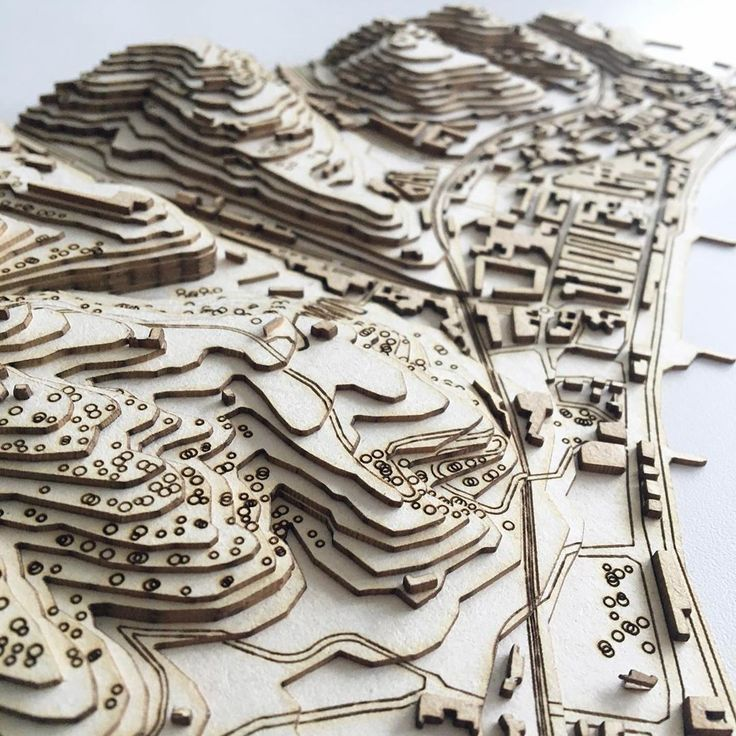
\includegraphics[width=0.7\textwidth]{chapters/120-topologie/images/relief.jpg}
\caption{Rekonstruktion einer Approximation der Topographie aus den
\index{Topographie}%
Höhenlinien mit Hilfe von Platten, die entlang der Höhenlinien ausgeschnitten
worden sind.
\label{buch:topologie:morse:fig:relief}}
\end{figure}
%
Aus einer glatten Funktion $f\colon M\to\mathbb{R}$ lässt
sich eine natürliche Zerlegung einer Mannigfaltigkeit konstruieren.
In Abbildung~\ref{buch:topologie:morse:fig:karte} zeigt eine 
topographische Karte.
Die Höhenlinien sind die Niveaulinien der Funktion, die einem
Punkt seine Höhe über dem Meeresspiegel zuordnet.
Die Höhenlinien zerlegen die Karte in Streifen, Ringe und andere
zweidimensionale Gebiete.
Der geübte Kartenleser ist in der Lage, aus den Höhenlinien eine
Vorstellung der Topographie zu rekonstruieren.
Man kann aber auch aus den Höhenlinien ein massstäbliches Modell
des Geländes rekonstruieren.
Für jedes Niveau schneidet man das von der Höhenlinie berandete Gebiet
aus einer Holzplatte aus und schichtet die erhaltenen Platten
wie in Abbildung~\ref{buch:topologie:morse:fig:relief} gezeigt
auf.
Es entsteht eine Approximation des Geländes.

Wir betrachten jetzt eine einzelne Höhenlinie.
Die Höhenlinie zur Höhe $c$ ist die Menge der Punkte
\[
H_c
=
\{ p\in M\mid f(p) = c \}.
\]
Wenn wir $c$ um einen kleinen Betrag $\Delta c$ verschiebt sich
die Höhenlinie in eine Richtung senkrecht auf die Höhenlinie.
Ein positives $\Delta c$ bedeutet, dass wir eine Höhenlinie weiter
oben am Berg suchen.
Ist $\Delta c$ klein genug, ist die neue Höhenlinie $H_{c+\Delta c}$
meistens eine Kurve, die in unmittelbarer Nähe der Kurve $H_c$.
die Veränderung von $c$ hat also keine wesentlichen Auswirkungen
auf die Gestalt der Höhenlinie, wenigstens wenn die Höhenlinie
immer an einem Hang entlang verläuft.

Die Voraussetzung, dass die Höhenlinie dem Hang entlang verlaufen
muss, damit einen kleine Höhenänderung keine Auswirkung auf die
Gestalt der Kurve hat, ist zum Beispiel bei einem Gipfel verletzt.
Sei $p$ ein lokales Maximum der Funktion $f$ und U eine so kleine
Umgebung von $p$, dass die Höhenlinie $H_c = \{p\}$ nur den Punkt $p$
enthält.
Vergrössert man $c$ um $\Delta c>0$, verschwindet der Punkt $p$,
die Höhenlinie $H_{c+\Delta c}=\emptyset$ ist leer.
Bei einer Verkleinerung wird wird die Höhenline $H_{c+\Delta c}$ zu
einer geschlossenen Kurve, die den Punkt $p$ umschliesst
(Abbildung~\ref{buch:topologie:morse:fig:karte}, Umgebung des Punktes 1384),
wenigstens wenn die zweiten Ableitungen von $f$ an der Stelle $p$
nicht verschwinden.

Ein ganz anderes Bild bietet sich bei einem Pass der Höhe $c$.
Auch ein Sattelpunkt der Fläche ist eine Stelle, an der
alle partiellen ersten Ableitungen verschwinden.
Die Menge $H_c$ besteht aber nicht aus einem Punkt, vielmehr
kommen im Punkt $p$ vier Höhenlinien zusammen.
Für grössere und kleiner Werte verschwindet der Schnittpunkt,
es bleiben zwei nicht verbundene Höhenlinie wie in
bei links unterhalb der Büelhöchi in
Abbildung~\ref{buch:topologie:morse:fig:karte}.

Diese Diskussion zeigt, dass wesentliche Eigenschaften der Topographie
aus Punkten abzulesen sind, an denen die ersten Ableitungen verschwinden,
die zweiten Ableitungen aber nicht (was das genau heisst, muss noch
definiert werden).

%
% Index einer Nullstelle
%
\subsection{Kritische Punkte und ihr Index}
In diesem Abschnitt ist $M$ eine $n$-dimensionale Mannigfaltigkeit.
Wir betrachten die Menge $C^\infty(M)$ der beliebig oft stetig
differenzierbare Funktionen auf $M$.

%
% Kritische Punkte
%
\subsubsection{Kritische Punkte}
Die äussere Ableitung einer Funktion $f\colon M\to\mathbb{R}$ 
wird ein einer Karte $\varphi_\alpha\colon U_\alpha\to\mathbb{R}^n$
zu einer Funktion der $n$ Koordinaten, die wir $f(x^1,\dots,x^n)$
schreiben.
Bei einem Maximum oder Minimum der Funktion verschwinden alle ersten
Ableitungen, in dieser Karte wird die äussere Ableitung
\[
df
=
\frac{\partial f}{\partial x^1}\,dx^1
+
\dots
+
\frac{\partial f}{\partial x^n}\,dx^n
=
0.
\]
Wechselt man das Koordinatensystem, ändert dies an der Tatsache, dass
$df=0$ ist, nichts.

\begin{definition}[kritischer Punkt]
\index{kritischer Punkt}%
\index{Punkt!kritisch}%
\index{kritischer Wert}%
\index{Wert!kritisch}%
Ein \emph{kritischer Punkt} einer glatten Funktion $f$ auf einer
differenzierbaren Mannigfaltigkeit ist ein Punkt $p\in M$, bei dem
$df(p)=0$ ist.
Der Wert $c=f(p)$ in einem kritischen Punkt $p$ heisst
\emph{kritischer Wert} der Funktion f.
\end{definition}

%
% Der Index eines kritischen Punktes
%
\subsubsection{Der Index eines kritischen Punktes}
Sei $p$ ein kritischer Punkt der Funktion $f$ auf der Mannigfaltigkeit $M$
mit dem kritischen Wert $c=f(p)$.
In einem Koordinatensystem in der Umgebung des Punktes $p$ kann die Funktion
durch die Taylor-Reihe 
\begin{align}
f(x^1,\dots,x^n)
&=
f(p)
+
\sum_{k=1}^n \frac{\partial f}{\partial x^k}(p) (x^k-x^k(p))
\\
&\qquad\mathstrut
+
\sum_{k,l=1}^n
\frac{\partial^2 f}{\partial x^k\,\partial x^l}(p)
(x^k-x^k(p))(x^l-x^l(p))
+
o(|x-p|^2)
\notag
\\
&=
c
+
\sum_{k,l=1}^n
\frac{\partial^2 f}{\partial x^k\,\partial x^l}(p)
(x^k-x^k(p))(x^l-x^l(p))
+
o(|x-p|^2)
\label{buch:topologie:morse:eqn:quadratisch}
\end{align}
approximiert werden.
Wir möchten sicherstellen, dass wir zuverlässige Aussagen über die
Form der \emph{Niveaumengen} $H_c=\{p\in M\mid f(p)=c\}$ machen können.
Dazu muss der quadratische Term in
\eqref{buch:topologie:morse:eqn:quadratisch}
immer gegenüber den Termen höherer Ordnung dominieren.
Dies ist nur möglich, wenn der quadratische Ausdruck
\[
H(v)
=
\sum_{k,l=1}^n
\frac{\partial^2 f}{\partial x^k\,\partial x^l}
v^k v^l
\]
nicht entartet ist.

\begin{definition}[entartete quadratische Form]
XXX
\end{definition}

Die Matrix $H$ mit den Einträgen
\[
h_{kl} = \frac{\partial f}{\partial x^k\,\partial x^l}
\]
ist in einem nicht entarteten kritischen Punkt eine symmetrische
Matrix.
Da symmetrische Matrizen durch orthogonale Transformationen
diagonalisierbar sind, können wir das Koorinatensystem mit
einer orthogonalen Matrix so drehen, dass $H$ die Form
\[
H(v)
=
\sum_{i=1}^n \lambda_i (v^i)^2
\]
bekommt.
Die $\lambda_i$ sind die Eigenwerte der Matrix $H$, keiner
der Eigenwerte verschwindet.
Durch Streckung der Koordinatenachse $x^1$ mit dem Faktor
$\!\sqrt{|\lambda_i|}$  mittels
$y^i = \!\sqrt{|\lambda_i|}x^i$ kann die Entwicklung
\eqref{buch:topologie:morse:eqn:quadratisch}
in die Form
\begin{align*}
f(y^1,\dots,y^n)
\\
&=
c
+
\operatorname{sgn}(\lambda_1)\,(y^1)^2
+
\dots
+
\operatorname{sgn}(\lambda_n)\,(y^n)^2.
\end{align*}
Es kommt also nur auf die Vorzeichen der Eigenwerte an.
Bei einem Koordinatenwechsel ändert sich die Matrix $H$ der zweiten
Ableitungen, aber die Anzahl der positiven und negativen Eigenwerte
bleibt erhalten.

\begin{definition}[Index]
\index{Index einer quadratischen Form}%
Der \emph{Index} einer nicht entarteten quadratischen Form ist die
Anzahl der negativen Eigenwerte.
\end{definition}

%
% Rekonstruktion
%
\subsection{Rekonstruktion}

%
% de Rham Kohomologie
%
\section{de Rham-Kohomologie}

\subsection{Zyklen und Ränder}

\subsection{Definition der Kohomologiegruppen}

%
% Beispiele
%
\subsection{Beispiele}

\subsubsection{Zusammenziehbarer Raum}

\subsubsection{Torus}

\subsubsection{Kugel}

